\documentclass{ximera}

\title{Strategic Coordinate Changes}
\author{Zack Reed}

\begin{document}
\begin{abstract}
In this activity we develop strategies for choosing between rectangular, cylindrical, and spherical coordinates, guided by the geometry of the integration region, and practice executing the full change-of-variables workflow from bounds to evaluation.
\end{abstract}
\maketitle


\section*{Strategic Coordinate Changes: From Cartesian to Spherical}

\begin{problem}
\textbf{Example: Region Between Curved Surfaces}

Find the mass of the solid bounded by the cone $z = \sqrt{x^2 + y^2}$ (below) and the sphere $x^2 + y^2 + z^2 = 4$ (above), with density $\delta(x,y,z) = z$ (denser at higher altitude).

We'll see that Cartesian coordinates produce a mess of nested square-root bounds, while spherical coordinates reduce each surface to a single constant equation.

\textbf{The Cone:} $z = \sqrt{x^2 + y^2}$

\begin{center}
\begin{tikzpicture}[x={(0.8cm,-0.4cm)}, y={(0.8cm,0.4cm)}, z={(0cm,1.1cm)}, scale=1.5]
    % Axes (shortened to reduce clutter)
    \draw[->] (0,0,0) -- (1.6,0,0) node[right,font=\small] {$x$};
    \draw[->] (0,0,0) -- (0,1.6,0) node[above,font=\small] {$y$};
    \draw[->] (0,0,0) -- (0,0,2.6) node[above,font=\small] {$z$};

    % Fill cone surface: quads between z and z+dz, theta and theta+30deg
    \foreach \z in {0.25,0.5,...,2.0} {
        \pgfmathsetmacro{\znext}{\z+0.25}
        \foreach \theta in {0,30,...,330} {
            \pgfmathsetmacro{\thetanext}{\theta+30}
            % Quad corners: (r,theta,z), (r+dr,theta,z+dz), (r+dr,theta+dth,z+dz), (r,theta+dth,z)
            \fill[orange!55!red, opacity=0.5]
                ({\z*cos(\theta)},{\z*sin(\theta)},{\z})
                -- ({\znext*cos(\theta)},{\znext*sin(\theta)},{\znext})
                -- ({\znext*cos(\thetanext)},{\znext*sin(\thetanext)},{\znext})
                -- ({\z*cos(\thetanext)},{\z*sin(\thetanext)},{\z}) -- cycle;
        }
    }

    % Key horizontal circles (just a few)
    \foreach \z in {0.7,1.414,2.0} {
        \draw[orange!80!black, thin, domain=0:360, samples=36, smooth, variable=\t]
            plot ({\z*cos(\t)}, {\z*sin(\t)}, {\z});
    }

    % Generating lines (8 directions)
    \foreach \theta in {0,45,...,315} {
        \draw[orange!50!black, thin] (0,0,0) -- ({2*cos(\theta)}, {2*sin(\theta)}, 2);
    }

    % Label (clear of geometry)
    \node[font=\small, align=left] at (-0.2, -0.8, 2.1) {$z=\sqrt{x^2+y^2}$};
    \node[font=\scriptsize, orange!70!black] at (0.5,0,0.3) {$\phi=\tfrac{\pi}{4}$ in spherical};
\end{tikzpicture}
\end{center}

\textbf{The Sphere:} $x^2 + y^2 + z^2 = 4$ (radius 2, centered at origin)

\begin{center}
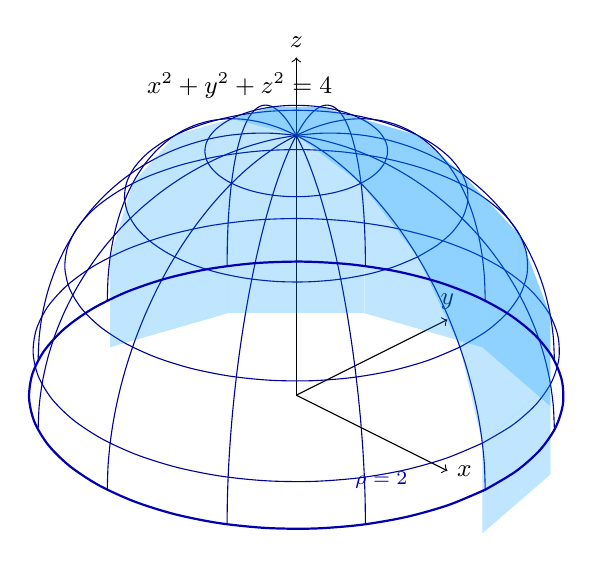
\begin{tikzpicture}[x={(0.8cm,-0.4cm)}, y={(0.8cm,0.4cm)}, z={(0cm,1.1cm)}, scale=1.5]
    % Axes
    \draw[->] (0,0,0) -- (1.6,0,0) node[right,font=\small] {$x$};
    \draw[->] (0,0,0) -- (0,1.6,0) node[above,font=\small] {$y$};
    \draw[->] (0,0,0) -- (0,0,2.6) node[above,font=\small] {$z$};

    % Upper hemisphere wireframe (latitude lines)
    \foreach \phi in {20,40,60,80} {
        \pgfmathsetmacro{\r}{2*sin(\phi)}
        \pgfmathsetmacro{\zz}{2*cos(\phi)}
        \draw[blue!60!black, thin, domain=0:360, samples=36, smooth, variable=\t]
            plot ({\r*cos(\t)}, {\r*sin(\t)}, {\zz});
    }
    % Longitude lines
    \foreach \theta in {0,30,...,330} {
        \draw[blue!55!black, thin, domain=0:90, samples=18, smooth, variable=\p]
            plot ({2*sin(\p)*cos(\theta)}, {2*sin(\p)*sin(\theta)}, {2*cos(\p)});
    }

    % Light fill on visible front face
    \foreach \phi in {0,20,...,80} {
        \pgfmathsetmacro{\phinext}{\phi+20}
        \pgfmathsetmacro{\ra}{2*sin(\phi)}
        \pgfmathsetmacro{\za}{2*cos(\phi)}
        \pgfmathsetmacro{\rb}{2*sin(\phinext)}
        \pgfmathsetmacro{\zb}{2*cos(\phinext)}
        \foreach \theta in {0,30,...,150} {
            \pgfmathsetmacro{\thetanext}{\theta+30}
            \fill[blue!40!cyan, opacity=0.25]
                ({\ra*cos(\theta)},{\ra*sin(\theta)},{\za})
                -- ({\rb*cos(\theta)},{\rb*sin(\theta)},{\zb})
                -- ({\rb*cos(\thetanext)},{\rb*sin(\thetanext)},{\zb})
                -- ({\ra*cos(\thetanext)},{\ra*sin(\thetanext)},{\za}) -- cycle;
        }
    }

    % Equator
    \draw[blue!70!black, thick, domain=0:360, samples=36, smooth, variable=\t]
        plot ({2*cos(\t)}, {2*sin(\t)}, 0);

    % Label
    \node[font=\small] at (0, -0.6, 2.6) {$x^2+y^2+z^2=4$};
    \node[font=\scriptsize, blue!70!black] at (1.0, -0.1, -0.25) {$\rho=2$};
\end{tikzpicture}
\end{center}

\textbf{The Intersection Region:} Between cone (below) and sphere (above)

\begin{center}
\begin{tikzpicture}[scale=1.6]
  % 2D cross-section in the x-z half-plane
  % Cone: z = x  (i.e., phi = pi/4)
  % Sphere: x^2 + z^2 = 4 (upper, z >= 0)
  % Intersection at x = z = sqrt(2) ~ 1.414

  % Fill the region between cone and sphere
  \fill[green!25, opacity=0.75]
    (0,0)
    -- plot[domain=0:1.414, samples=30, variable=\x] (\x, \x)
    -- plot[domain=1.414:0, samples=30, variable=\x] (\x, {sqrt(4-\x*\x)})
    -- cycle;

  % Draw cone line
  \draw[orange!70!black, very thick, domain=0:1.55, samples=2]
    plot (\x, \x) node[right, font=\small, orange!80!black]{cone: $\phi=\tfrac{\pi}{4}$};

  % Draw sphere arc
  \draw[blue!70!black, very thick, domain=0:2.0, samples=40]
    plot (\x, {sqrt(4-\x*\x)}) node[above right=-2pt, font=\small, blue!80!black]{sphere: $\rho=2$};

  % Axes
  \draw[->] (-0.15,0) -- (2.4,0) node[right, font=\small]{$x$ (or $r$)};
  \draw[->] (0,-0.15) -- (0,2.5) node[above, font=\small]{$z$};

  % Intersection point
  \fill[purple] (1.414,1.414) circle (1.5pt);
  \draw[purple, dashed] (1.414,0) -- (1.414,1.414) -- (0,1.414);
  \node[below, font=\scriptsize] at (1.414,-0.08) {$\sqrt{2}$};
  \node[left, font=\scriptsize] at (-0.06,1.414) {$\sqrt{2}$};

  % rho = 2 arc dimension
  \draw[violet, <->, thick] (0,0) -- ({2*cos(22)},{2*sin(22)})
    node[midway, above left=-2pt, font=\scriptsize, violet]{$\rho=2$};

  % phi angle
  \draw[orange!80!black, ->] (0,0.55)
    arc[start angle=90, delta angle=-45, radius=0.55]
    node[midway, right, font=\scriptsize, orange!80!black]{$\phi$};

  % Region label
  \node[green!50!black, font=\small] at (0.45, 1.55) {Our};
  \node[green!50!black, font=\small] at (0.45, 1.32) {Region};

  % Note about revolution
  \node[font=\scriptsize, gray!70, align=center] at (1.7, 0.3)
    {(rotate around\\$z$-axis for 3D region)};
\end{tikzpicture}
\end{center}

\textbf{Step 1: Understanding the Cartesian Challenge}

The cone and sphere intersect where $z = \sqrt{x^2+y^2}$ and $x^2+y^2+z^2=4$.

Substituting: $x^2+y^2+(\sqrt{x^2+y^2})^2 = 4$, so $2(x^2+y^2) = 4$, giving $x^2+y^2 = \answer{2}$.

At the intersection: $z = \sqrt{2}$ and the circle has radius $\sqrt{2}$.

\textbf{In Cartesian coordinates with order $dz\,dy\,dx$:}

For fixed $(x,y)$ with $x^2+y^2 \leq 2$:
$$\sqrt{x^2+y^2} \leq z \leq \sqrt{4-x^2-y^2}$$

For fixed $x$: $-\sqrt{2-x^2} \leq y \leq \sqrt{2-x^2}$

Overall: $-\sqrt{2} \leq x \leq \sqrt{2}$

$$M = \int_{-\sqrt{2}}^{\sqrt{2}} \int_{-\sqrt{2-x^2}}^{\sqrt{2-x^2}} \int_{\sqrt{x^2+y^2}}^{\sqrt{4-x^2-y^2}} z\,dz\,dy\,dx$$

This is quite messy! Square roots everywhere, and the bounds depend on each other in complicated ways.

\textbf{Step 2: Recognizing the Pattern}

What features suggest a better coordinate system?
\begin{selectAll}
    \choice[correct]{The sphere equation is $x^2 + y^2 + z^2 = 4$ (radial from origin)}
    \choice[correct]{The cone equation involves $\sqrt{x^2 + y^2}$ (cylindrical symmetry)}
    \choice[correct]{Both surfaces are centered at the origin}
    \choice{The region is rectangular}
\end{selectAll}

For a sphere centered at the origin, which coordinate system is best?
\begin{multipleChoice}
    \choice{Cartesian}
    \choice{Cylindrical}
    \choice[correct]{Spherical}
\end{multipleChoice}

\textbf{Why spherical coordinates?  A side-by-side comparison of the bounds.}

\begin{center}
\begin{tikzpicture}[scale=1.0]

%=== LEFT: 3D oblique view of the cone+sphere bounded region ===
\begin{scope}[x={(0.85cm,-0.38cm)}, y={(0.85cm,0.38cm)}, z={(0cm,1.05cm)}, xshift=0.3cm, yshift=0.2cm]
  % First octant view: phi in [0,45deg], theta in [0,90deg], rho in [0,2]

  % Fill region on sphere surface (phi 0..45, bands by phi)
  \foreach \phA in {0,15,30} {
    \pgfmathsetmacro{\phB}{\phA+15}
    \foreach \thA in {0,30,60} {
      \pgfmathsetmacro{\thB}{\thA+30}
      \pgfmathsetmacro{\ra}{2*sin(\phA)} \pgfmathsetmacro{\za}{2*cos(\phA)}
      \pgfmathsetmacro{\rb}{2*sin(\phB)} \pgfmathsetmacro{\zb}{2*cos(\phB)}
      \fill[green!30!white,opacity=0.60]
        ({\ra*cos(\thA)},{\ra*sin(\thA)},\za)
        -- ({\rb*cos(\thA)},{\rb*sin(\thA)},\zb)
        -- ({\rb*cos(\thB)},{\rb*sin(\thB)},\zb)
        -- ({\ra*cos(\thB)},{\ra*sin(\thB)},\za) -- cycle;
    }
  }

  % Fill cone cap (phi=45, rho 0..2, theta 0..90)
  \foreach \thA in {0,30,60} {
    \pgfmathsetmacro{\thB}{\thA+30}
    \foreach \rhoA in {0,0.7,1.4} {
      \pgfmathsetmacro{\rhoB}{\rhoA+0.7}
      \fill[orange!25!white,opacity=0.55]
        ({\rhoA*sin(45)*cos(\thA)},{\rhoA*sin(45)*sin(\thA)},{\rhoA*cos(45)})
        -- ({\rhoA*sin(45)*cos(\thB)},{\rhoA*sin(45)*sin(\thB)},{\rhoA*cos(45)})
        -- ({\rhoB*sin(45)*cos(\thB)},{\rhoB*sin(45)*sin(\thB)},{\rhoB*cos(45)})
        -- ({\rhoB*sin(45)*cos(\thA)},{\rhoB*sin(45)*sin(\thA)},{\rhoB*cos(45)}) -- cycle;
    }
  }

  % Sphere wireframe lines
  \foreach \ph in {15,30,45} {
    \pgfmathsetmacro{\rr}{2*sin(\ph)}
    \pgfmathsetmacro{\zz}{2*cos(\ph)}
    \draw[blue!55!black,thin,domain=0:90,smooth,samples=10,variable=\t]
      plot ({\rr*cos(\t)},{\rr*sin(\t)},\zz);
  }
  \foreach \th in {0,30,60,90} {
    \draw[blue!55!black,thin,domain=0:45,smooth,samples=9,variable=\p]
      plot ({2*sin(\p)*cos(\th)},{2*sin(\p)*sin(\th)},{2*cos(\p)});
  }

  % Sphere boundary arcs (2 visible edges at theta=0 and theta=90)
  \draw[blue!70!black,very thick,domain=0:90,smooth,samples=12,variable=\p]
    plot ({2*sin(\p)},0,{2*cos(\p)});
  \draw[blue!70!black,very thick,domain=0:90,smooth,samples=12,variable=\p]
    plot (0,{2*sin(\p)},{2*cos(\p)});

  % Cone boundary arcs and lines
  \draw[orange!80!black,very thick,domain=0:90,smooth,samples=12,variable=\t]
    plot ({sqrt(2)*cos(\t)},{sqrt(2)*sin(\t)},{sqrt(2)});
  \draw[orange!75!black,thick] (0,0,0) -- ({sqrt(2)},0,{sqrt(2)});
  \draw[orange!75!black,thick] (0,0,0) -- (0,{sqrt(2)},{sqrt(2)});

  % Axes
  \draw[->,gray!60] (0,0,0) -- (2.4,0,0) node[right,font=\scriptsize]{$x$};
  \draw[->,gray!60] (0,0,0) -- (0,2.4,0) node[right,font=\scriptsize]{$y$};
  \draw[->,gray!60] (0,0,0) -- (0,0,2.5) node[above,font=\scriptsize]{$z$};

  % Surface labels
  \node[orange!75!black,font=\scriptsize,align=left] at (0.9,0.9,1.6)
    {cone\\$\phi\!=\!\tfrac{\pi}{4}$};
  \node[blue!65!black,font=\scriptsize] at (0.25,0.25,2.2) {sphere $\rho\!=\!2$};
  \node[green!50!black,font=\scriptsize] at (0.55,0.55,1.4) {region};

  % Messy bounds annotation (compact, below)
  \node[font=\tiny,align=center,red!65!black] at (1.2,0,-0.55)
    {$-\sqrt{2}\le x\le\sqrt{2}$,\; $-\sqrt{2-x^2}\le y\le\sqrt{2-x^2}$,\;
     $\sqrt{x^2+y^2}\le z\le\sqrt{4-x^2-y^2}$};

  \node[font=\small,align=center] at (1.2,0,-0.95)
    {\textbf{Cartesian:} 3D region, nested bounds};
\end{scope}

%=== ARROW ===
\begin{scope}[xshift=4.1cm,yshift=1.7cm]
  \draw[->,very thick,gray!60](0,0)--(1.0,0);
  \node[gray!60,font=\scriptsize,align=center] at (0.5,-0.3){switch to\\spherical};
\end{scope}

%=== RIGHT: Spherical bounds --- clean rectangle in (rho, phi) space ===
\begin{scope}[xshift=5.5cm]
  \draw[->](-0.2,0)--(3.5,0) node[right,font=\small]{$\rho$};
  \draw[->](0,-0.2)--(0,3.5) node[above,font=\small]{$\phi$};

  % In spherical: rho in [0,2], phi in [0, pi/4]
  % pi/4 ~ 0.785 rad -> scale phi*3.5/(pi/2) ~ phi*2.23 for display
  \def\phiscale{2.4}  % scale factor: pi/4 -> 1.88 display units
  \def\phimax{1.88}   % = (pi/4)*phiscale
  \def\rhomax{3.2}    % display width for rho=2: scale 2->3.2

  % The region is just a RECTANGLE in spherical space!
  \fill[green!25,opacity=0.8] (0,0) rectangle (\rhomax,\phimax);
  \draw[blue!70!black,very thick] (0,0) rectangle (\rhomax,\phimax);

  % Labels on sides
  \draw[<->,blue!60!black,thick] (0,-0.28)--(\rhomax,-0.28)
        node[midway,below,font=\small]{$\rho: 0\to 2$};
  \draw[<->,blue!60!black,thick] (-0.3,0)--(-0.3,\phimax)
        node[midway,left,font=\small]{$\phi: 0\to\pi/4$};

  % Sphere label
  \draw[blue!70!black,very thick] (\rhomax,-0.08)--(\rhomax,\phimax+0.08);
  \node[blue!70!black,font=\small,right] at (\rhomax+0.05,\phimax/2) {sphere};
  \node[blue!70!black,font=\tiny,right] at (\rhomax+0.05,\phimax/2-0.3) {$\rho=2$};

  % Cone label
  \draw[orange!70!black,very thick] (-0.08,\phimax)--(\rhomax+0.08,\phimax);
  \node[orange!70!black,font=\small,above] at (\rhomax/2,\phimax+0.05) {cone: $\phi=\pi/4$};

  % theta is free
  \node[font=\scriptsize,gray!70,align=center] at (\rhomax/2,\phimax/2)
        {$\theta: 0\to 2\pi$\\(free, by symmetry)};

  % Annotation box
  \draw[green!50!black,rounded corners,thick] (-0.55,-0.55) rectangle ({\rhomax+0.7},{\phimax+0.55});
  \node[green!50!black,font=\scriptsize,align=center] at ({\rhomax/2},-0.42)
        {all bounds are constants!};

  \node[font=\small,align=center,below] at ({\rhomax/2},-0.7)
        {\textbf{Spherical:} constant bounds, clean rectangle};
\end{scope}

\end{tikzpicture}
\end{center}

The two diagrams above say it all: on the left the integration region sits inside a 3D tangle of square roots; on the right those same surfaces become the single constant equations $\rho=2$ (sphere) and $\phi=\pi/4$ (cone).  The parameter-space region is a plain rectangle, and the $\theta$-integral contributes only a factor of $2\pi$.

\textbf{Step 3: The Spherical Coordinate Transformation}

Spherical coordinates $(\rho, \phi, \theta)$ relate to Cartesian via:
\begin{align*}
x &= \rho\sin\phi\cos\theta\\
y &= \rho\sin\phi\sin\theta\\
z &= \rho\cos\phi
\end{align*}

where:
\begin{itemize}
    \item $\rho \geq 0$ is the distance from the origin
    \item $0 \leq \phi \leq \pi$ is the angle down from the positive $z$-axis
    \item $0 \leq \theta < 2\pi$ is the azimuthal angle (same as cylindrical)
\end{itemize}

Key relation: $x^2 + y^2 + z^2 = \answer{\rho^2}$

The volume element transforms: $dV = \answer{\rho^2 \sin\phi}\,d\rho\,d\phi\,d\theta$

\textbf{Step 4: Transform the Surfaces}

\textbf{The sphere:} $x^2 + y^2 + z^2 = 4$ becomes $\rho^2 = 4$, so $\rho = \answer{2}$

This is beautiful! A constant bound.

\textbf{The cone:} $z = \sqrt{x^2 + y^2}$

Using $z = \rho\cos\phi$ and $\sqrt{x^2+y^2} = \rho\sin\phi$:
$$\rho\cos\phi = \rho\sin\phi$$

Dividing by $\rho$: $\cos\phi = \sin\phi$, so $\tan\phi = 1$, giving $\phi = \answer{\pi/4}$

The cone is a constant angle! The region is between the cone ($\phi = \pi/4$) and the north pole ($\phi = 0$).

So: $0 \leq \phi \leq \answer{\pi/4}$

\textbf{Step 5: Transform the Density}

The density was $\rho(x,y,z) = z$

In spherical coordinates: $z = \rho\cos\phi$

So the density becomes: $\rho(\rho,\phi,\theta) = \answer{\rho\cos\phi}$

(Note: We're using $\rho$ for both the density function and the spherical coordinate. Context makes it clear!)

\textbf{Step 6: Set Up the Integral in Spherical Coordinates}

The bounds are:
\begin{itemize}
    \item $0 \leq \rho \leq 2$ (from origin to sphere)
    \item $0 \leq \phi \leq \pi/4$ (from $z$-axis to cone)
    \item $0 \leq \theta \leq 2\pi$ (full rotation)
\end{itemize}

$$M = \int_{\answer{0}}^{\answer{2\pi}} \int_{\answer{0}}^{\answer{\pi/4}} \int_{\answer{0}}^{\answer{2}} (\rho\cos\phi) \cdot \rho^2\sin\phi\,d\rho\,d\phi\,d\theta$$

Simplifying: 
$$M = \int_0^{2\pi} \int_0^{\pi/4} \int_0^2 \rho^3\cos\phi\sin\phi\,d\rho\,d\phi\,d\theta$$

\textbf{Step 7: Evaluate the Integral}

The variables separate! Let's do each integral:

\textbf{Inner integral ($\rho$):}
$$\int_0^2 \rho^3\,d\rho = \left[\frac{\rho^4}{4}\right]_0^2 = \frac{16}{4} = \answer{4}$$

\textbf{Middle integral ($\phi$):}
$$\int_0^{\pi/4} \cos\phi\sin\phi\,d\phi = \int_0^{\pi/4} \frac{1}{2}\sin(2\phi)\,d\phi$$
$$= \frac{1}{2}\left[-\frac{1}{2}\cos(2\phi)\right]_0^{\pi/4} = -\frac{1}{4}[\cos(\pi/2) - \cos(0)]$$
$$= -\frac{1}{4}[0 - 1] = \answer{1/4}$$

\textbf{Outer integral ($\theta$):}
$$\int_0^{2\pi} d\theta = \answer{2\pi}$$

\textbf{Final answer:}
$$M = 4 \cdot \frac{1}{4} \cdot 2\pi = \answer{2\pi}$$

\begin{feedback}
Compare the two approaches! In Cartesian coordinates, we had:
\begin{itemize}
    \item Square root bounds: $-\sqrt{2-x^2} \leq y \leq \sqrt{2-x^2}$
    \item Nested dependence of bounds
    \item Complex expressions like $\sqrt{4-x^2-y^2}$
\end{itemize}

In spherical coordinates, we had:
\begin{itemize}
    \item Constant bounds: $0 \leq \rho \leq 2$, $0 \leq \phi \leq \pi/4$, $0 \leq \theta \leq 2\pi$
    \item Separable integral
    \item The sphere became $\rho = 2$ (one equation!)
    \item The cone became $\phi = \pi/4$ (one equation!)
\end{itemize}

This is the power of choosing the right coordinate system! The geometry of the problem guides us to the natural coordinates.
\end{feedback}
\end{problem}


\section*{Choosing the Right Coordinate System}

\begin{center}
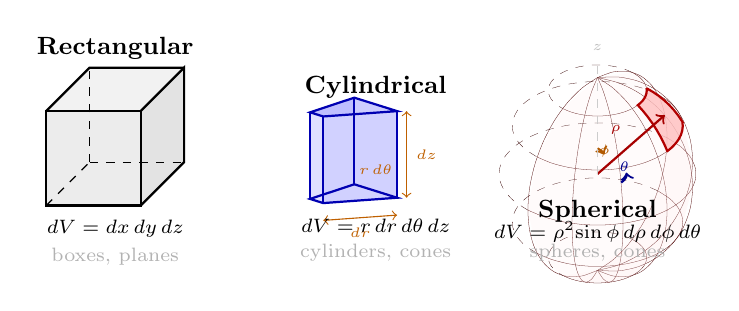
\begin{tikzpicture}[scale=1.0]

%=== LEFT: Rectangular ===
\begin{scope}[xshift=0cm]
  % Draw a box (oblique 3D projection)
  \def\W{1.2} \def\H{1.2} \def\D{0.55}
  \fill[gray!15] (0,0) rectangle (\W,\H);
  \fill[gray!22] (\W,0) -- ({\W+\D},\D) -- ({\W+\D},{\H+\D}) -- (\W,\H) -- cycle;
  \fill[gray!10] (0,\H) -- (\D,{\H+\D}) -- ({\W+\D},{\H+\D}) -- (\W,\H) -- cycle;
  \draw[black,thick] (0,0) rectangle (\W,\H);
  \draw[black,thick] (\W,0) -- ({\W+\D},\D) -- ({\W+\D},{\H+\D}) -- (\W,\H);
  \draw[black,thick] (0,\H) -- (\D,{\H+\D}) -- ({\W+\D},{\H+\D});
  \draw[black,dashed] (0,0) -- (\D,\D); \draw[black,dashed] (\D,\D) -- ({\W+\D},\D);
  \draw[black,dashed] (\D,\D) -- (\D,{\H+\D});

  \node[font=\small,align=center] at ({(\W+\D)/2},{\H+\D+0.25}) {\textbf{Rectangular}};
  \node[font=\scriptsize,align=center] at ({(\W+\D)/2},-0.3)
    {$dV=dx\,dy\,dz$};
  \node[font=\scriptsize,gray!60,align=center] at ({(\W+\D)/2},-0.65)
    {boxes, planes};
\end{scope}

%=== CENTER: Cylindrical (wedge piece) ===
\begin{scope}[xshift=3.1cm]
  \def\rI{0.4} \def\rO{1.3} \def\thA{20} \def\thB{70} \def\hz{1.1}
  \pgfmathsetmacro{\pILx}{\rI*cos(\thA)+0.3*\rI*sin(\thA)}
  \pgfmathsetmacro{\pILy}{0.22*\rI*sin(\thA)}
  \pgfmathsetmacro{\pIRx}{\rI*cos(\thB)+0.3*\rI*sin(\thB)}
  \pgfmathsetmacro{\pIRy}{0.22*\rI*sin(\thB)}
  \pgfmathsetmacro{\pOLx}{\rO*cos(\thA)+0.3*\rO*sin(\thA)}
  \pgfmathsetmacro{\pOLy}{0.22*\rO*sin(\thA)}
  \pgfmathsetmacro{\pORx}{\rO*cos(\thB)+0.3*\rO*sin(\thB)}
  \pgfmathsetmacro{\pORy}{0.22*\rO*sin(\thB)}
  \pgfmathsetmacro{\pILyt}{\pILy+\hz}
  \pgfmathsetmacro{\pIRyt}{\pIRy+\hz}
  \pgfmathsetmacro{\pOLyt}{\pOLy+\hz}
  \pgfmathsetmacro{\pORyt}{\pORy+\hz}
  \pgfmathsetmacro{\pOLytlbl}{\pOLy+\hz+0.3}
  \pgfmathsetmacro{\pOLymid}{(\pOLy+\pORy)/2}
  \pgfmathsetmacro{\pORxmid}{(\pOLx+\pORx)/2}

  % Bottom face
  \fill[blue!15]
    (\pILx,\pILy) -- (\pOLx,\pOLy) -- (\pORx,\pORy) -- (\pIRx,\pIRy) -- cycle;
  % Top face
  \fill[blue!25]
    (\pILx,\pILyt) -- (\pOLx,\pOLyt) -- (\pORx,\pORyt) -- (\pIRx,\pIRyt) -- cycle;
  % Outer side
  \fill[blue!20]
    (\pOLx,\pOLy) -- (\pORx,\pORy) -- (\pORx,\pORyt) -- (\pOLx,\pOLyt) -- cycle;
  % Inner side (visible)
  \fill[blue!12]
    (\pILx,\pILy) -- (\pIRx,\pIRy) -- (\pIRx,\pIRyt) -- (\pILx,\pILyt) -- cycle;
  % Left radial side
  \fill[blue!18]
    (\pILx,\pILy) -- (\pOLx,\pOLy) -- (\pOLx,\pOLyt) -- (\pILx,\pILyt) -- cycle;
  % Draw edges
  \draw[blue!70!black,thick]
    (\pILx,\pILy) -- (\pOLx,\pOLy) -- (\pORx,\pORy) -- (\pIRx,\pIRy) -- cycle;
  \draw[blue!70!black,thick]
    (\pILx,\pILyt) -- (\pOLx,\pOLyt) -- (\pORx,\pORyt) -- (\pIRx,\pIRyt) -- cycle;
  \draw[blue!70!black,thick] (\pILx,\pILy)--(\pILx,\pILyt);
  \draw[blue!70!black,thick] (\pOLx,\pOLy)--(\pOLx,\pOLyt);
  \draw[blue!70!black,thick] (\pORx,\pORy)--(\pORx,\pORyt);
  \draw[blue!70!black,thick] (\pIRx,\pIRy)--(\pIRx,\pIRyt);

  % Dimension labels
  \draw[<->,orange!75!black,thin]
    (\pILx,{\pILy-0.22}) -- (\pOLx,{\pOLy-0.22})
    node[midway,below,font=\tiny]{$dr$};
  \draw[<->,orange!75!black,thin]
    ({\pOLx+0.12},\pOLy) -- ({\pOLx+0.12},\pOLyt)
    node[midway,right,font=\tiny]{$dz$};
  \node[orange!75!black,font=\tiny,above] at (\pORxmid,\pORy)
    {$r\,d\theta$};

  \node[font=\small,align=center] at (\pORxmid,\pOLytlbl) {\textbf{Cylindrical}};
  \node[font=\scriptsize,align=center] at (\pORxmid,{\pOLy-0.35})
    {$dV=r\,dr\,d\theta\,dz$};
  \node[font=\scriptsize,gray!60,align=center] at (\pORxmid,{\pOLy-0.7})
    {cylinders, cones};
\end{scope}

%=== RIGHT: Spherical — actual 3D sphere with wedge ===
\begin{scope}[x={(0.52cm,-0.27cm)}, y={(0.52cm,0.27cm)}, z={(0cm,0.72cm)}, xshift=7.0cm, yshift=0.4cm]
  \def\RS{1.7}
  % Front hemisphere wireframe (thin — more lines for rounder sphere)
  \foreach \ph in {30,60,90,120,150} {
    \pgfmathsetmacro{\rr}{\RS*sin(\ph)} \pgfmathsetmacro{\zz}{\RS*cos(\ph)}
    \draw[red!30!black,ultra thin,domain=-90:90,smooth,samples=15,variable=\t]
      plot ({\rr*cos(\t)},{\rr*sin(\t)},\zz);
  }
  \foreach \th in {-90,-60,-30,0,30,60,90} {
    \draw[red!30!black,ultra thin,domain=0:180,smooth,samples=15,variable=\p]
      plot ({\RS*sin(\p)*cos(\th)},{\RS*sin(\p)*sin(\th)},{\RS*cos(\p)});
  }
  % Back hemisphere (dashed)
  \foreach \ph in {30,60,90,120,150} {
    \pgfmathsetmacro{\rr}{\RS*sin(\ph)} \pgfmathsetmacro{\zz}{\RS*cos(\ph)}
    \draw[red!20!black,ultra thin,dashed,domain=90:270,smooth,samples=15,variable=\t]
      plot ({\rr*cos(\t)},{\rr*sin(\t)},\zz);
  }
  % Light fill
  \foreach \ph in {0,30,...,150} {
    \pgfmathsetmacro{\phn}{\ph+30}
    \pgfmathsetmacro{\ra}{\RS*sin(\ph)} \pgfmathsetmacro{\za}{\RS*cos(\ph)}
    \pgfmathsetmacro{\rb}{\RS*sin(\phn)} \pgfmathsetmacro{\zb}{\RS*cos(\phn)}
    \foreach \th in {-90,-60,...,60} {
      \pgfmathsetmacro{\thn}{\th+30}
      \fill[red!10!white,opacity=0.15]
        ({\ra*cos(\th)},{\ra*sin(\th)},\za)
        -- ({\rb*cos(\th)},{\rb*sin(\th)},\zb)
        -- ({\rb*cos(\thn)},{\rb*sin(\thn)},\zb)
        -- ({\ra*cos(\thn)},{\ra*sin(\thn)},\za) -- cycle;
    }
  }

  % Highlighted dV wedge (rho=RS, phi 30..60, theta 10..50) — curved on sphere surface
  \def\phA{30} \def\phB{60} \def\thA{10} \def\thB{50}
  % Curved surface patch: 4 arc edges (follows sphere curvature)
  \fill[red!25,opacity=0.80]
    plot[domain=\phA:\phB,samples=8,variable=\p]
      ({\RS*sin(\p)*cos(\thA)},{\RS*sin(\p)*sin(\thA)},{\RS*cos(\p)})
    -- plot[domain=\thA:\thB,samples=8,variable=\t]
      ({\RS*sin(\phB)*cos(\t)},{\RS*sin(\phB)*sin(\t)},{\RS*cos(\phB)})
    -- plot[domain=\phB:\phA,samples=8,variable=\p]
      ({\RS*sin(\p)*cos(\thB)},{\RS*sin(\p)*sin(\thB)},{\RS*cos(\p)})
    -- plot[domain=\thB:\thA,samples=8,variable=\t]
      ({\RS*sin(\phA)*cos(\t)},{\RS*sin(\phA)*sin(\t)},{\RS*cos(\phA)})
    -- cycle;
  \draw[red!70!black,thick]
    plot[domain=\phA:\phB,samples=8,variable=\p]
      ({\RS*sin(\p)*cos(\thA)},{\RS*sin(\p)*sin(\thA)},{\RS*cos(\p)})
    -- plot[domain=\thA:\thB,samples=8,variable=\t]
      ({\RS*sin(\phB)*cos(\t)},{\RS*sin(\phB)*sin(\t)},{\RS*cos(\phB)})
    -- plot[domain=\phB:\phA,samples=8,variable=\p]
      ({\RS*sin(\p)*cos(\thB)},{\RS*sin(\p)*sin(\thB)},{\RS*cos(\p)})
    -- plot[domain=\thB:\thA,samples=8,variable=\t]
      ({\RS*sin(\phA)*cos(\t)},{\RS*sin(\phA)*sin(\t)},{\RS*cos(\phA)})
    -- cycle;

  % rho vector
  \pgfmathsetmacro{\phM}{(\phA+\phB)/2}
  \pgfmathsetmacro{\thM}{(\thA+\thB)/2}
  \draw[red!65!black,thick,->] (0,0,0)
    -- ({\RS*sin(\phM)*cos(\thM)},{\RS*sin(\phM)*sin(\thM)},{\RS*cos(\phM)})
    node[midway,above left,font=\tiny,red!65!black]{$\rho$};

  % phi arc
  \draw[orange!70!black,thick,->]
    ({0.45*sin(0)*cos(\thM)},{0.45*sin(0)*sin(\thM)},{0.45*cos(0)})
    arc[start angle=90,delta angle={-\phA},radius=0.45];
  \node[orange!70!black,font=\tiny] at ({0.3*sin(\phM/2)*cos(\thM)},{0.3*sin(\phM/2)*sin(\thM)},{0.45*cos(\phM/2)}) {$\phi$};

  % theta arc
  \draw[blue!55!black,thick,->]
    ({0.5*cos(\thA)},{0.5*sin(\thA)},0)
    arc[start angle=\thA,end angle=\thB,radius=0.5];
  \node[blue!55!black,font=\tiny] at ({0.48*cos(\thM)},{0.48*sin(\thM)},0.2) {$\theta$};

  \draw[gray!40,dashed,thin] (0,0,0) -- (0,0,{\RS+0.3}) node[above,font=\tiny,gray!50]{$z$};

  \node[font=\small,align=center] at (0,0,-0.65) {\textbf{Spherical}};
  \node[font=\scriptsize,align=center] at (0,0,-1.02)
    {$dV=\rho^2\!\sin\phi\,d\rho\,d\phi\,d\theta$};
  \node[font=\scriptsize,gray!60,align=center] at (0,0,-1.38)
    {spheres, cones};
\end{scope}

\end{tikzpicture}
\end{center}

\begin{problem}
Match each region type with the best coordinate system:

For a cylinder aligned with the $z$-axis:
\begin{multipleChoice}
    \choice{Rectangular}
    \choice[correct]{Cylindrical}
    \choice{Spherical}
\end{multipleChoice}

For a sphere centered at the origin:
\begin{multipleChoice}
    \choice{Rectangular}
    \choice{Cylindrical}
    \choice[correct]{Spherical}
\end{multipleChoice}

For a rectangular box:
\begin{multipleChoice}
    \choice[correct]{Rectangular}
    \choice{Cylindrical}
    \choice{Spherical}
\end{multipleChoice}

For a cone:
\begin{multipleChoice}
    \choice{Rectangular}
    \choice{Cylindrical}
    \choice[correct]{Either cylindrical or spherical work well}
\end{multipleChoice}

\begin{feedback}
Choose coordinates that match your region's symmetry! This makes bounds simpler and integrals easier to evaluate.
\end{feedback}
\end{problem}


\end{document}
